
%%%%%%%%%%%%%%%%%%%

\chapter{Charlie in the design framework}
\label{chapter:charlieDesign}

The robot Charlie, introduced in chapter \ref{chapter:background}, was developed specifically for use by children with autism in communication therapy. Charlie is situated into the design framework introduced in chapter \ref{chapter:design}, in order to showcase how the framework defines an existing robot, based on the implementation detailed in the newest study \cite{boccanfuso2017low}. This is depicted in figure \ref{fig:charlieDesign}.

Charlie has been used to play interactive games with children with autism \cite{charlie2011, boccanfuso2017low}. It can be used to play with one child, or two at a time, which is why two different user quantities are indicated in figure \ref{fig:charlieDesign}. Leadership is also defined as mutual and alternate, as the robot explains the rules, but the child leads the interaction. Goals are mixed, since the game is a task to complete, but the child can lead the game in an exploratory manner.

The movement quality was estimated from photos of Charlie's mechanics, which do not afford organic movement. Social awareness was also estimated from the script provided in the study, which detailed Charlie saying hello and goodbye upon the child entering and leaving the interaction \cite{boccanfuso2017low}. The study also described Charlie being controlled by a human, but having machine vision to recognize successful imitation, which is why its autonomy is classified as partial \cite{boccanfuso2017low}.

\begin{figure}
\centering
  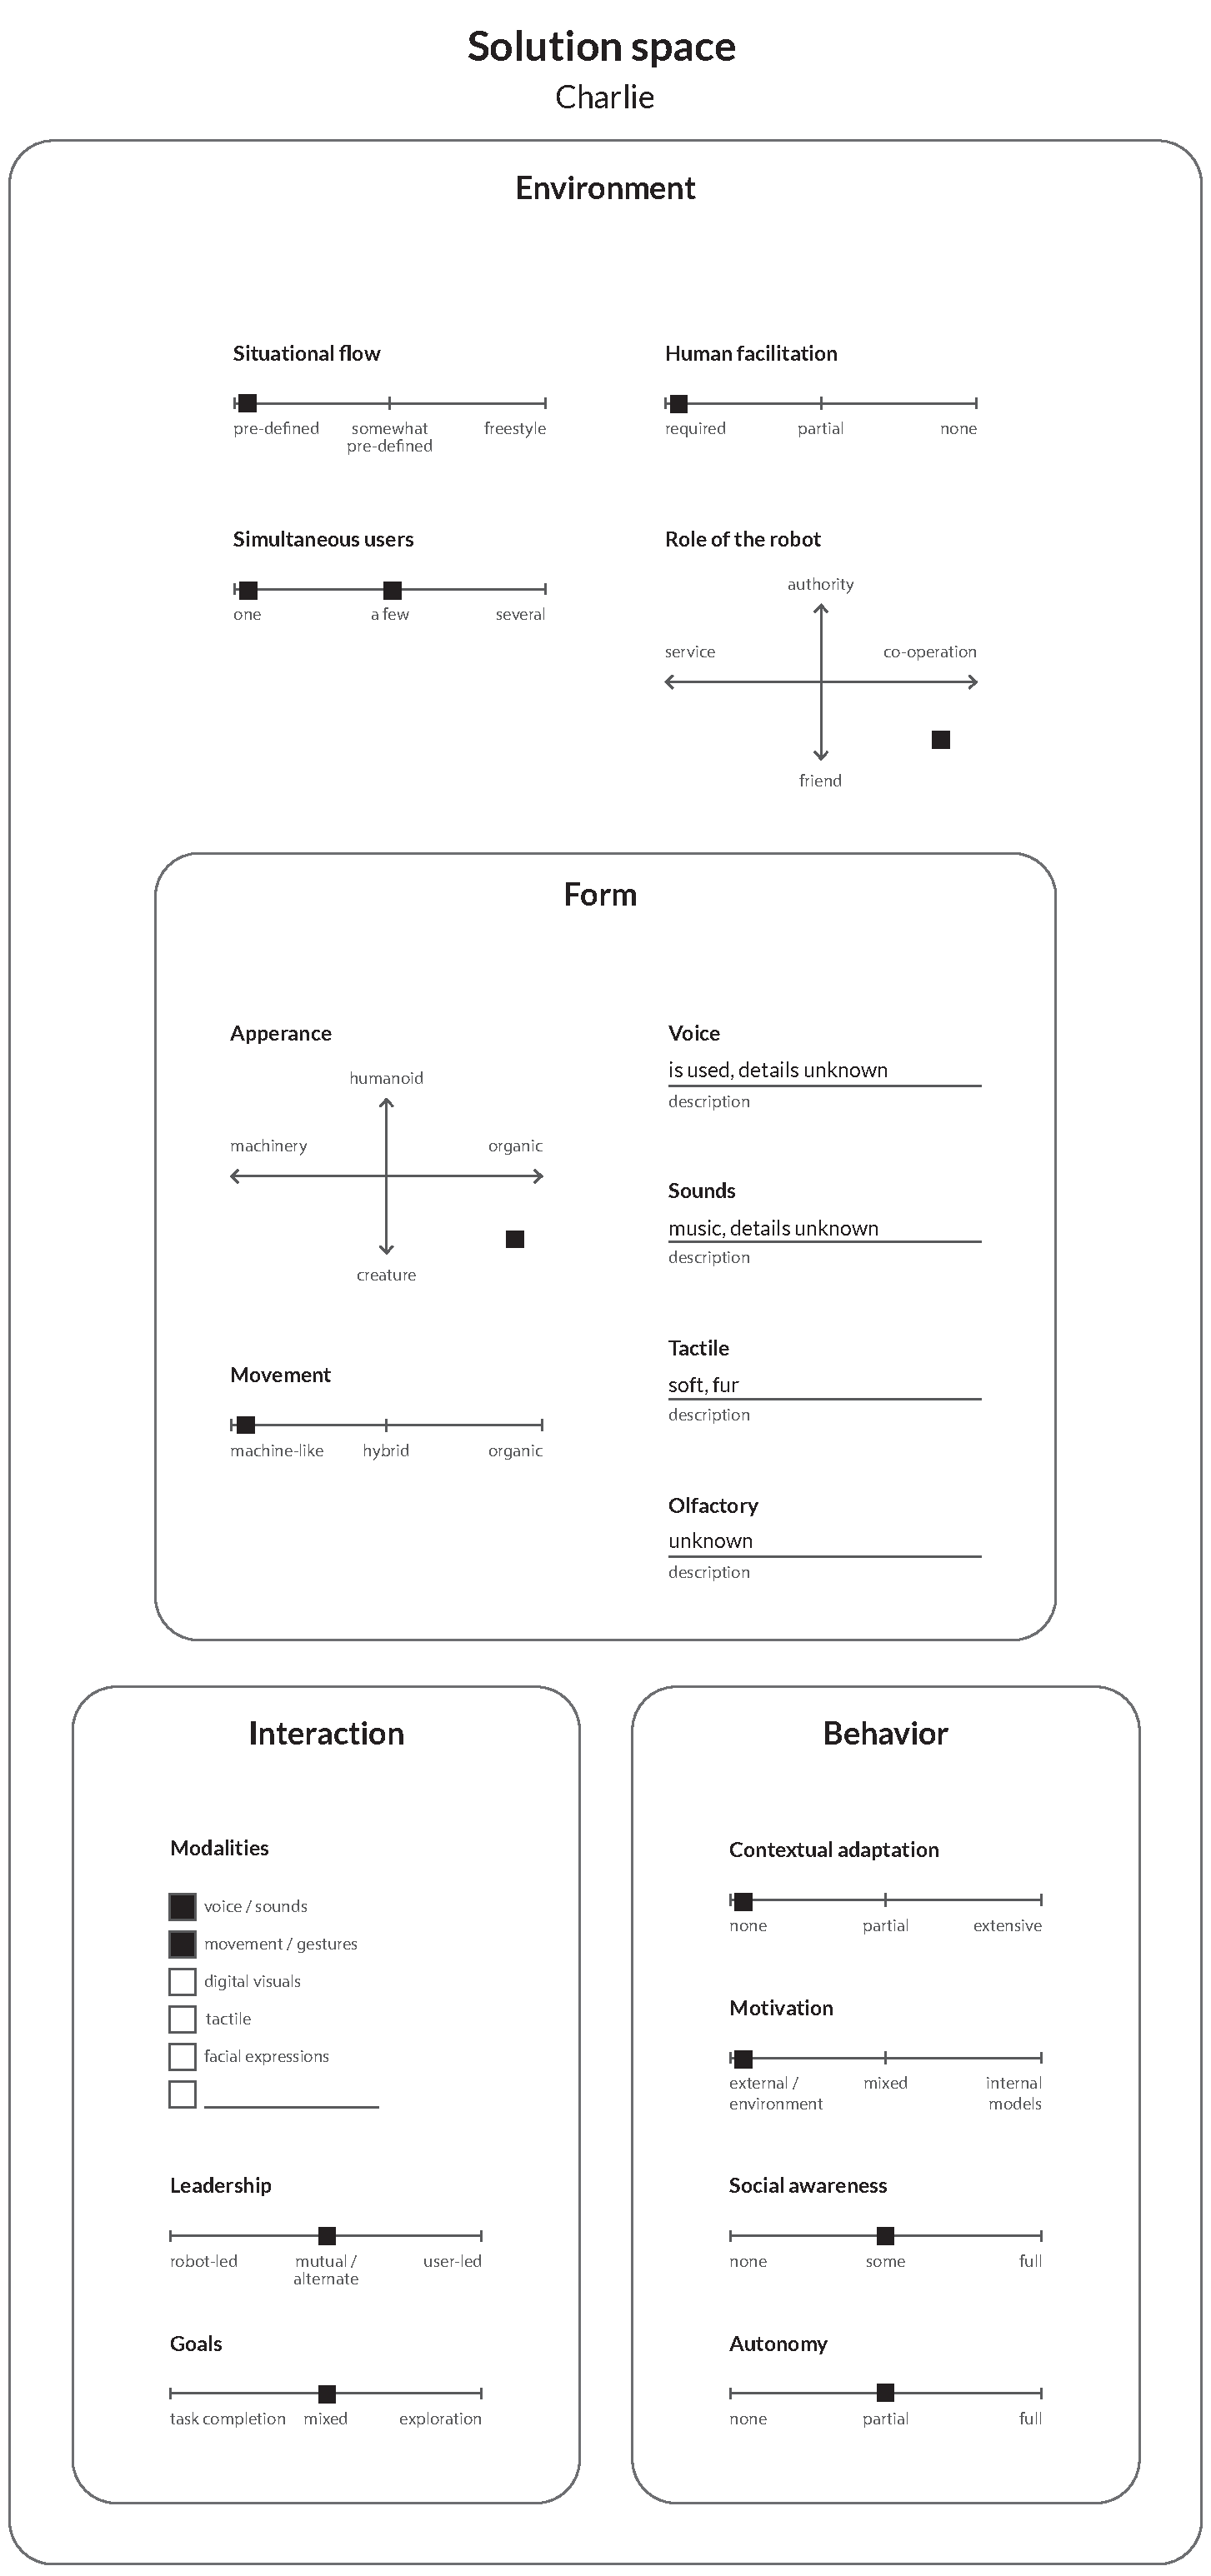
\includegraphics[scale=0.40]{images/solution_charlie-01.pdf}
  \caption{The robot Charlie is situated into the design framework.}
  \label{fig:charlieDesign}
\end{figure}

%%%%%%%%%%%%%

\chapter{Keepon in the design framework}
\label{chapter:keeponDesign}

The robot Keepon, introduced in chapter \ref{chapter:background}, was developed to study human-robot interaction with children, and was adapted to study interaction with children with autism. Keepon is situated into the design framework introduced in chapter \ref{chapter:design}, in order to showcase how the framework defines an existing robot, which was not designed specifically for use by children with autism. The implementation depicted in the framework (figure \ref{fig:keeponDesign} is based on the most recent study \cite{kozima2009keepon}.

The situational flow is described as freestyle, in contrast to both the InMoov described in this thesis and Charlie, which is detailed in chapter \ref{chapter:charlieDesign}. The Keepon was placed into a daycare for children with special needs, and autistic children could interact with it there sporadically. The study does not describe adults or other humans guiding the children to use the robot, but the Keepon was deliberately placed in the daycare among other toys. This means that there was partial human facilitation in the environment. The kids could explore the robot by themselves, or a few children could interact with it simultaneously. Children may also have interacted with the Keepon with their parent, or with a therapist.

The Keepon's form and manner of communication are very creature-like. It does not speak, and interacts by making chirping sounds, and moving to express its emotions. The Keepon's movements are quite organic, and do not appear robotic. 

The interactions were user-led, as the study did not detail Keepon initiating interactions \cite{kozima2009keepon}. The goal was for children to explore how the robot responds to them, meaning that goals were exploratory, and motivation for the robot's behavior was external. The study does not mention the robot exhibiting any improvisational behavior. The robot could operate both in an autonomous manner, or be fully controlled by a human, although the researchers mention that usually it was controlled by a human in studies with autistic children. No mention of the robot's socially aware qualities are made in the study \cite{kozima2009keepon}.





\begin{figure}
\centering
  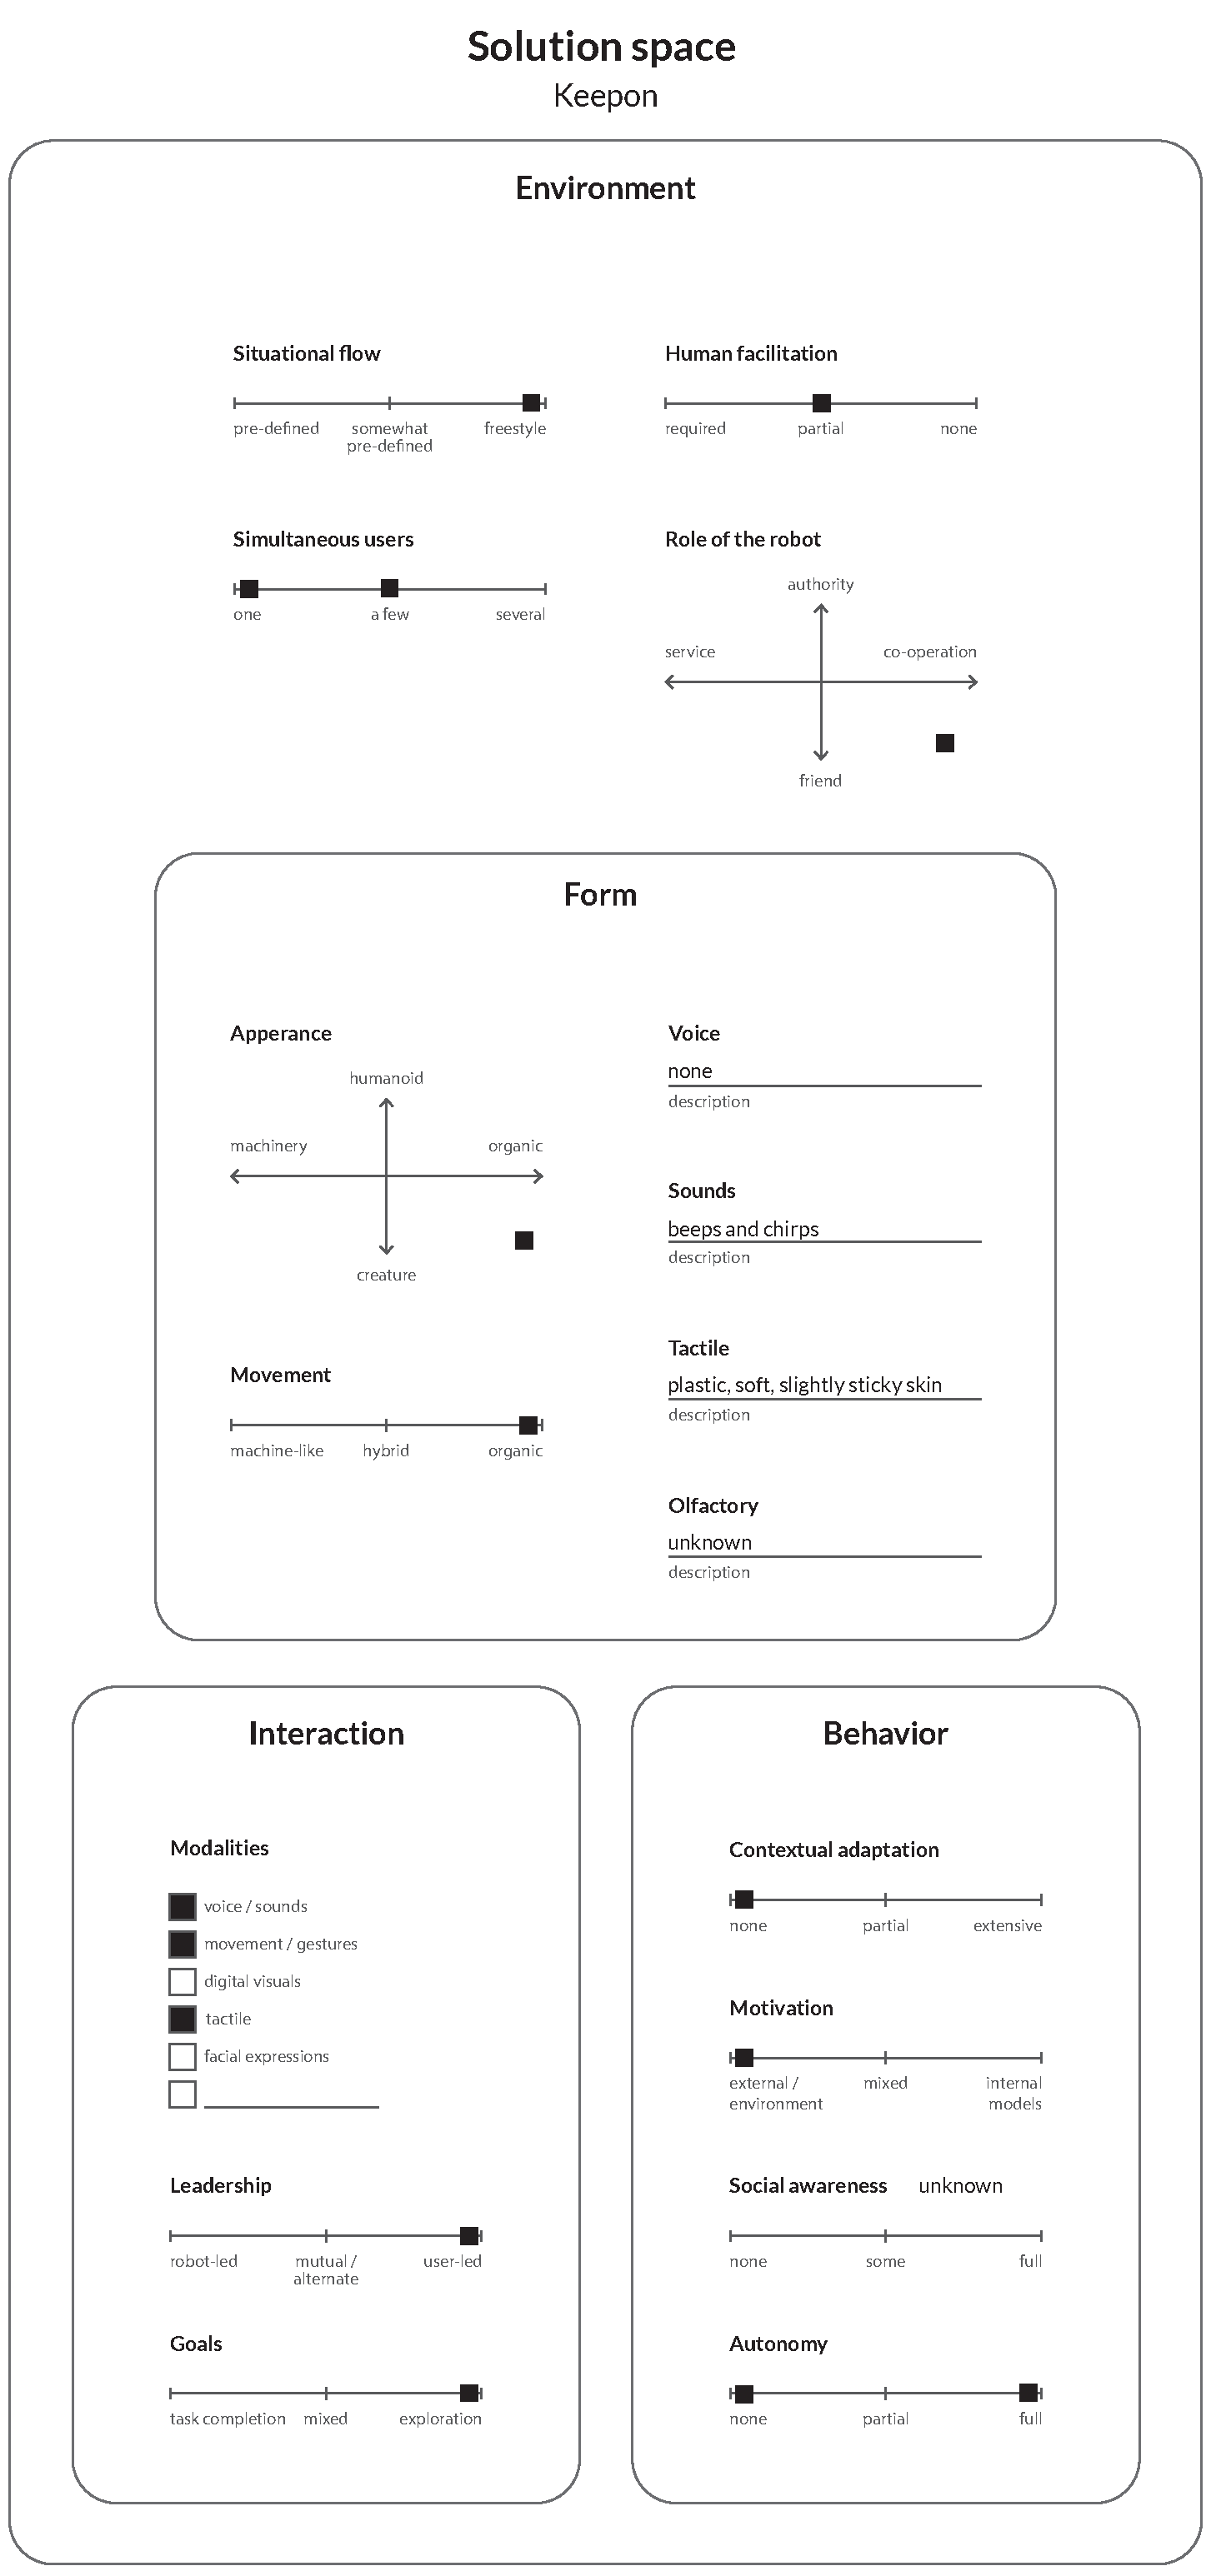
\includegraphics[scale=0.40]{images/solution_keepon-01.pdf}
  \caption{The robot Keepon is situated into the design framework.}
  \label{fig:keeponDesign}
\end{figure}

%%%%%%%%%%%%%%


\chapter{Explanation for children}
\label{chapter:explanation}

An explanation of the events to take place before, during and after the experiments was provided at the start of the experiment by the speech therapist. The symbols used are PECS-images, which are symbols frequently used by people with ASDs to communicate. The meaning of the images are written in Finnish below them.

\begin{figure}
\centering
  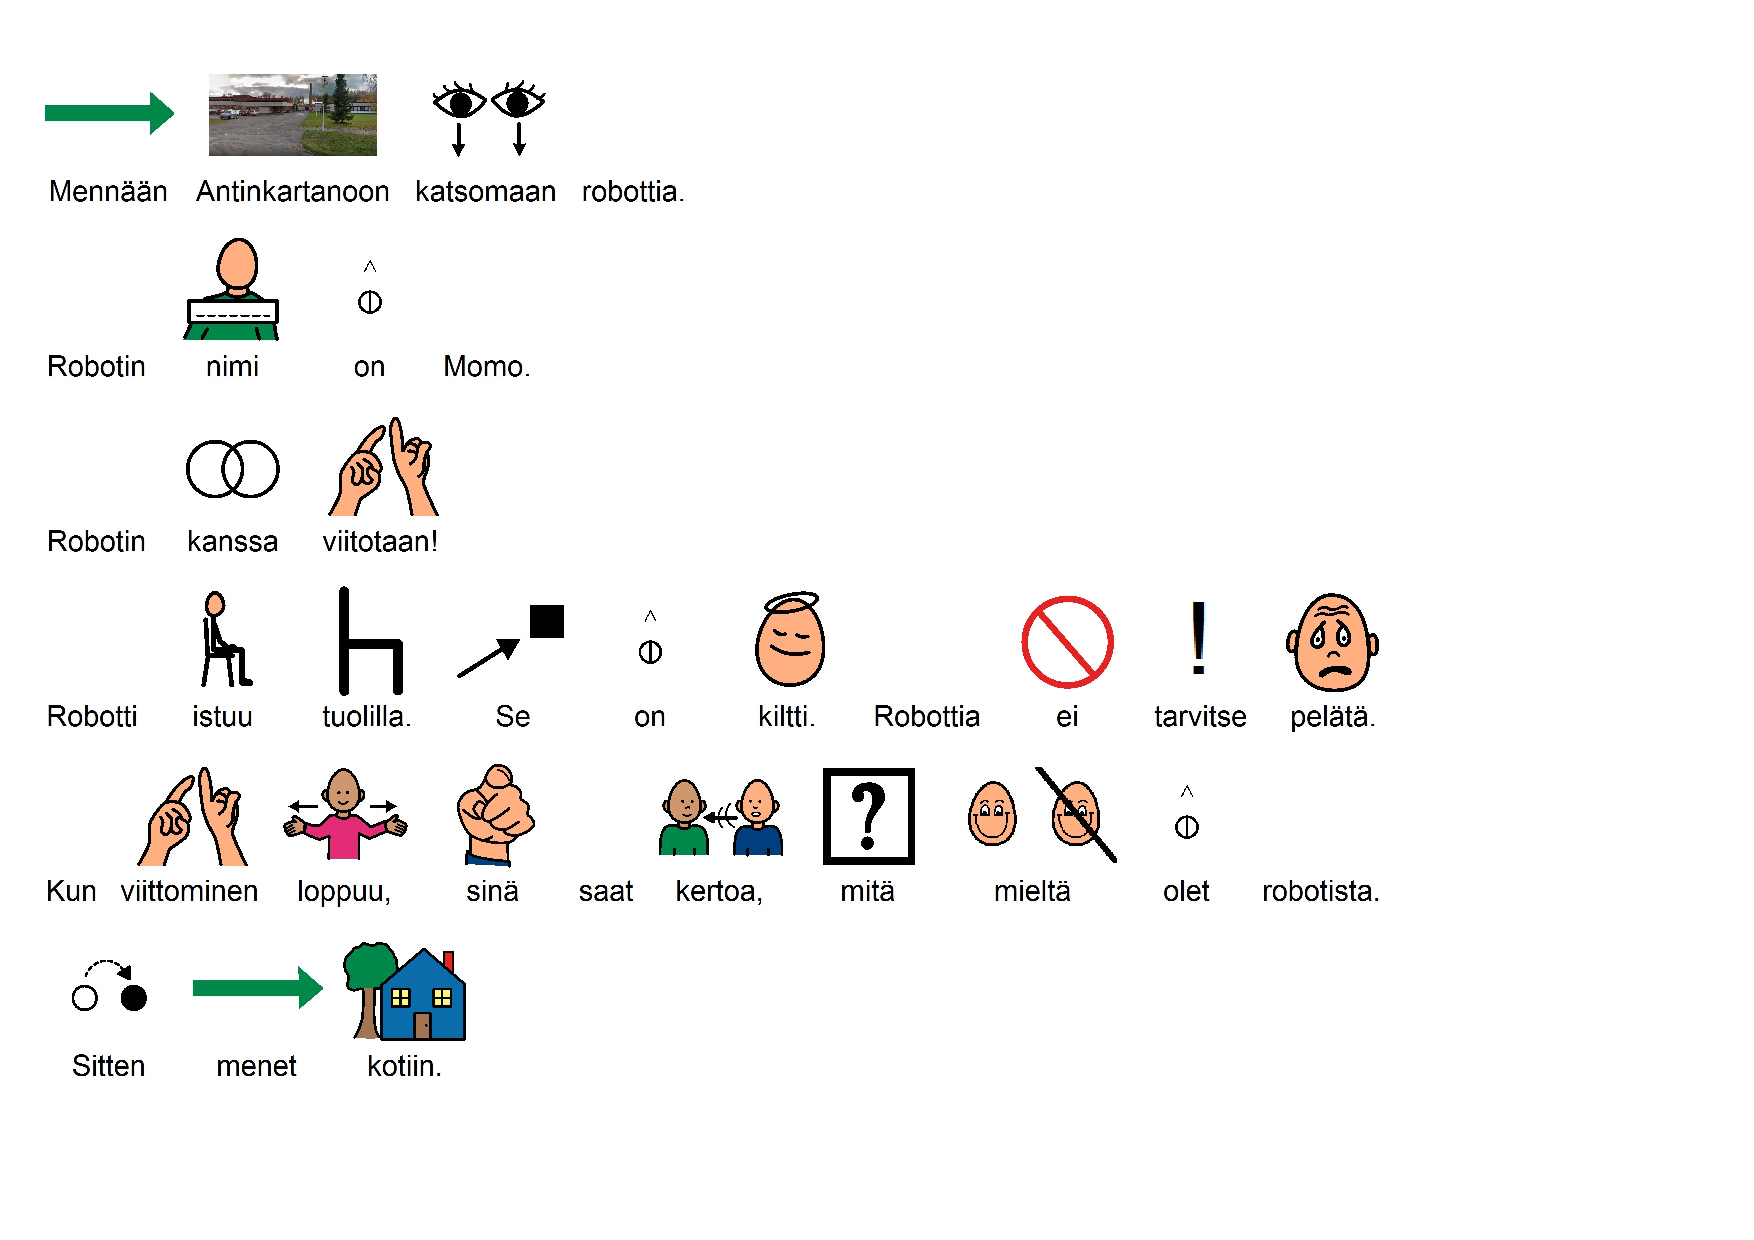
\includegraphics[scale=0.60, angle=-90]{images/kirje_lapselle.pdf}
  \caption{Explanation of the experiments for the children.}
  \label{fig:kirjelapselle}
\end{figure}



%%%



\chapter{Robot and child model conversation transcript}
\label{chapter:conversation}


\section{Esittely}
\begin{tabular}{llp{10cm}}
 1. & Robotti: & Hei, olen Momo. Olen robotti. \\
 2. &   & *robotti heiluttaa kättä tervehtimisen merkiksi* \\
 3. & Robotti: & Mikä sinun nimesi on? \\
 4. & Lapsi: & (nimi).\\
 5. & Robotti: & Hei, (nimi).\\
 6. & Robotti: & Tehdään yhdessä tehtäviä.\\
 7. & Robotti: & Katso, mitä minä teen. Tee sama perässä.\\
\end{tabular}

\section{Robotin viittoma}
\begin{tabular}{llp{10cm}}
 1. &  & *robotti viittoo* \\
 2. & & *jos tarve, robotti vilkuttaa valoa, tai näyttää tabletista kuvan* \\
 3. & Robotti: & (viittoman sana). \\
 4. & Robotti: & Nyt on sinun vuorosi. Tee samoin. \\
\end{tabular}


\section{Robotin reaktio}

Lapsi viittoo joko viittoo oikein, viittoo väärin, tai ei reagoi.

\subsection{Lapsi viittoo oikein}
\begin{tabular}{llp{10cm}}
 1. &  & *robotti näyttää peukkua ylös* \\
 2. & Robotti: & Hyvä, oikein meni.\\
 3. & Robotti: & Kokeillaan seuraavaa viittomaa.  \\
\end{tabular}

%%

\subsection{Lapsi viittoo väärin}
\begin{tabular}{llp{10cm}}
 1. & Robotti: & Hyvä yritys, ei mennyt ihan oikein. \\
 2. & Robotti: & Kokeillaan uudestaan. \\
 3. & & *robotti viittoo* \\
 4. & & *jos tarve, robotti vilkuttaa valoa, tai näyttää tabletista kuvan* \\
 5. & Robotti: & (viittoman sana). \\
 6. & Robotti: & Nyt on sinun vuorosi. Tee samoin. \\
 7. & & *odotetaan puheterapeutin indikoima aika* \\
\end{tabular}

\subsubsection{Lapsi viittoo nyt oikein}
\begin{tabular}{llp{10cm}}
 1. &  & *robotti näyttää peukkua ylös* \\
 2. & Robotti: & Hyvä, oikein meni.\\
 3. & Robotti: & Kokeillaan seuraavaa viittomaa.  \\
\end{tabular}

\subsubsection{Lapsi viittoo uudelleen väärin, tai ei reagoi}
\begin{tabular}{llp{10cm}}
 1. & Robotti: & Akuliina auttaa sinua nyt.\\
 2. & & *puheterapeutti näyttää viittoman, tai auttaa lasta tekemään sen kädestä pitäen* \\
 3. & Robotti: & Noin, nythän se onnistui.\\
 4. & Robotti: & Kokeillaan seuraavaa viittomaa.  \\
\end{tabular} \hfill\break

Joissakin tapauksissa lapsi ei saanut puheterapeutin avulla viittomaa oikein, jolloin repliikki 3 jätettiin sanomatta, ja siirrytiin suoraan repliikkiin 4.

%%

\subsection{Lapsi ei reagoi}
\begin{tabular}{llp{10cm}}
 1. & Robotti: & Hei, toista perässä mitä teen.. \\
 2. & & *robotti viittoo* \\
 3. & & *jos tarve, robotti vilkuttaa valoa, tai näyttää tabletista kuvan* \\
 4. & Robotti: & (viittoman sana). \\
 5. & Robotti: & Nyt on sinun vuorosi. Tee samoin. \\
 6. & & *odotetaan puheterapeutin indikoima aika* \\
\end{tabular}

\subsubsection{Lapsi viittoo nyt oikein}
\begin{tabular}{llp{10cm}}
 1. &  & *robotti näyttää peukkua ylös* \\
 2. & Robotti: & Hyvä, oikein meni.\\
 3. & Robotti: & Kokeillaan seuraavaa viittomaa.  \\
\end{tabular}

\subsubsection{Lapsi viittoo väärin, tai ei reagoi}
\begin{tabular}{llp{10cm}}
 1. & Robotti: & Akuliina auttaa sinua nyt.\\
 2. & & *puheterapeutti näyttää viittoman, tai auttaa lasta tekemään sen kädestä pitäen* \\
 3. & Robotti: & Noin, nythän se onnistui.\\
 4. & Robotti: & Kokeillaan seuraavaa viittomaa.  \\
\end{tabular} \hfill \break

Joissakin tapauksissa lapsi ei saanut puheterapeutin avulla viittomaa oikein, jolloin repliikki 3 jätettiin sanomatta, ja siirrytiin suoraan repliikkiin 4.

%%%

\section{Hyvästely}


\begin{tabular}{llp{10cm}}
 1. & Robotti: & Kiitos, minulla oli hauskaa.\\
 2. &  & *robotti heiluttaa kättää hyvästelemisen merkiksi*\\
 3. & Robotti: & Hei hei!  \\
\end{tabular}


%%%

\chapter{Survey for children}
\label{chapter:children}

After the experiments, the neurospychologist entered the experimentation room, and asked children to answer simple questions with the help of PECS-images.

\begin{figure}
\centering
  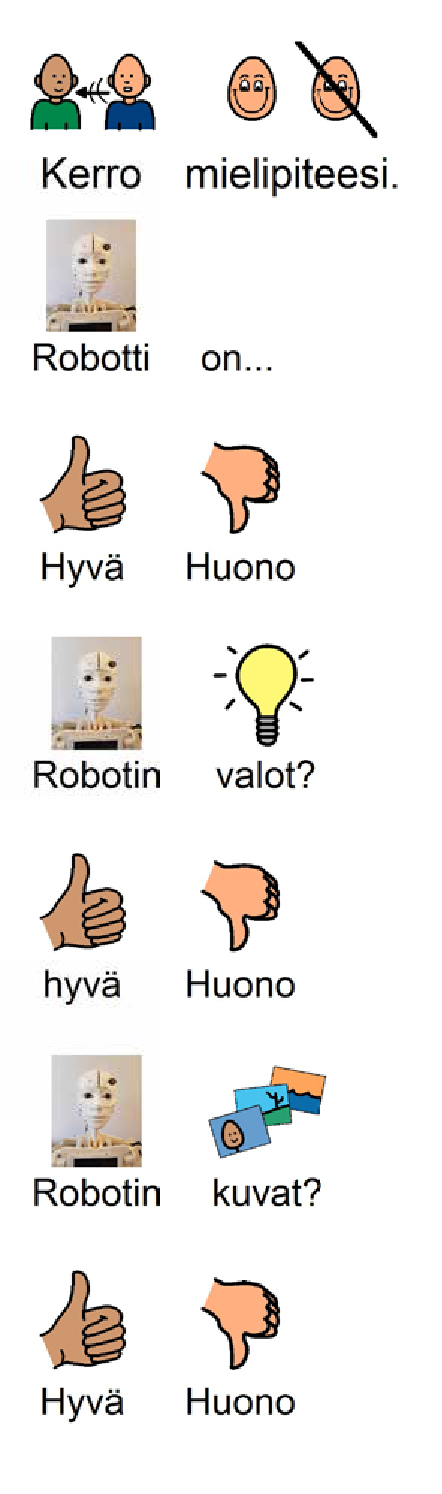
\includegraphics[scale=0.60]{images/kysely_lapselle_1.pdf}
  \caption{The first part of the survey for the children. The questions are: "Give your opinion." "The robot is... Good or bad?", "The robot's lights are... Good or bad?", "The robot's images are... Good or bad?"}
  \label{fig:kirjelapselle1}
\end{figure}

\begin{figure}
\centering
  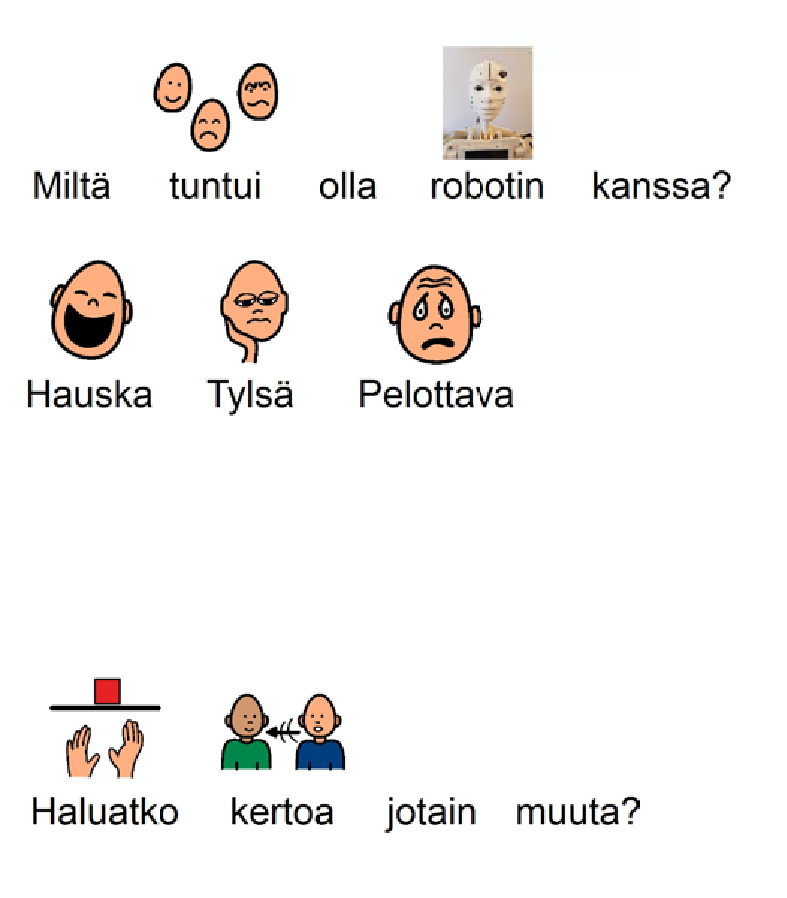
\includegraphics[scale=0.60]{images/kysely_lapselle_2.pdf}
  \caption{The second part of the survey for the children. The questions are: "How did it feel to be with the robot? Fun, boring, or scary?", "Do you want to tell something else?"}
  \label{fig:kirjelapselle2}
\end{figure}


%%%


\chapter{Survey for companions}
\label{chapter:companions}

After the experiments, the childrens' companions were given a survey to fill out. Some of the companions filled it immediately, and some returned it later by post. Companions were either childrens' parents, or therapists familiar with them. The surveys are in Finnish.

The questions are:
\begin{itemize}
  \item How did your child experience the situation? Fun, scary, boring, something else?
  \item How did you feel during the experiment? Fun, scary, boring, something else?
  \item Did you think your child had a connection with the robot? Yes or no.
  \item How did you perceive your child to have a connection with the robot when compared to a human? Better than with a human, same as with a human, worse than with a human.
  \item Do you think your child could benefit from practicing with the robot?
  \item Why or why not?
  \item What was the best and worst design condition (1. for best, 3. for worst)? Sign + sound, sign + sound + lights, sign + sound + image.
  \item What did you think of the design conditions? What was good and what was bad? Why? Sign + sound, sign + sound + lights, sign + sound + image.
  \item Do you have other things to say about the design conditions?
  \item Free word.
\end{itemize}

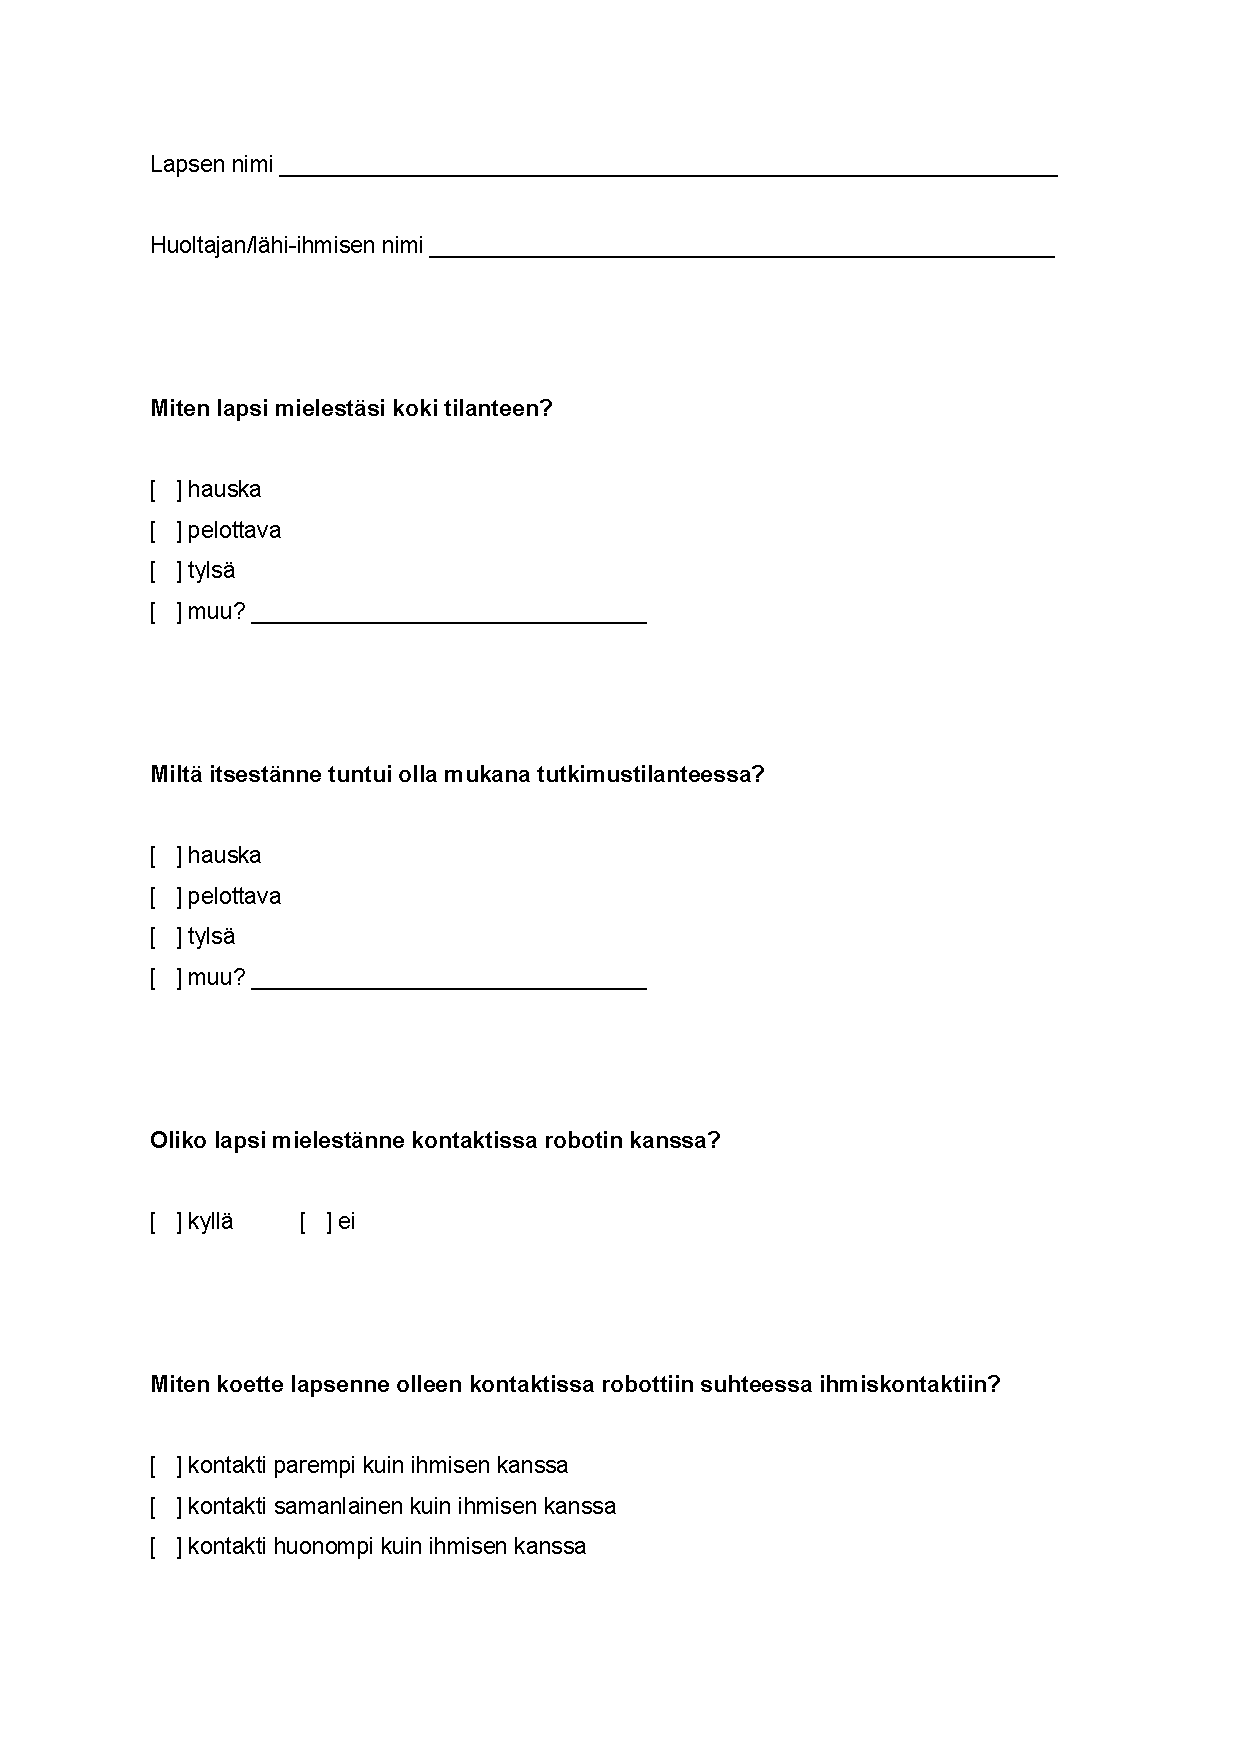
\includepdf[pages=-]{images/kysely_vanhemmille.pdf}


%%%

%For now, the Aalto logo variants are shown in Figure~\ref{fig:aaltologo}.

%\begin{figure}
%\begin{center}
%\subfigure[In English]{
\includegraphics[width=.8\textwidth]{images/aalto-logo-en}}
%\subfigure[Suomeksi]{
\includegraphics[width=.8\textwidth]{images/aalto-logo-fi}}
%\subfigure[På svenska]{
\includegraphics[width=.8\textwidth]{images/aalto-logo-se}}
%\caption{Aalto logo variants}
%\label{fig:aaltologo}
%\end{center}
%\end{figure}
